\documentclass[english]{exercisesheet}

\usepackage{bm}
\usepackage{mymath}
\usepackage{graphicx}
\usepackage{float}
\usepackage{amsbsy}
\usepackage{fixmath}
\usepackage{amsmath}

\author{Daniel Strenger, Lorenzo Minneci}
\immatriculationnumber{01531211, 11939539}
\semester{SS 2020}
\subject{Machine Learning}
\sheetnumber{3}

\begin{document}
 \makedocumentheader
  \begin{nexercise}{Datasets}
      \begin{solution} 1.
        \begin{figure}[H]
        \centering
        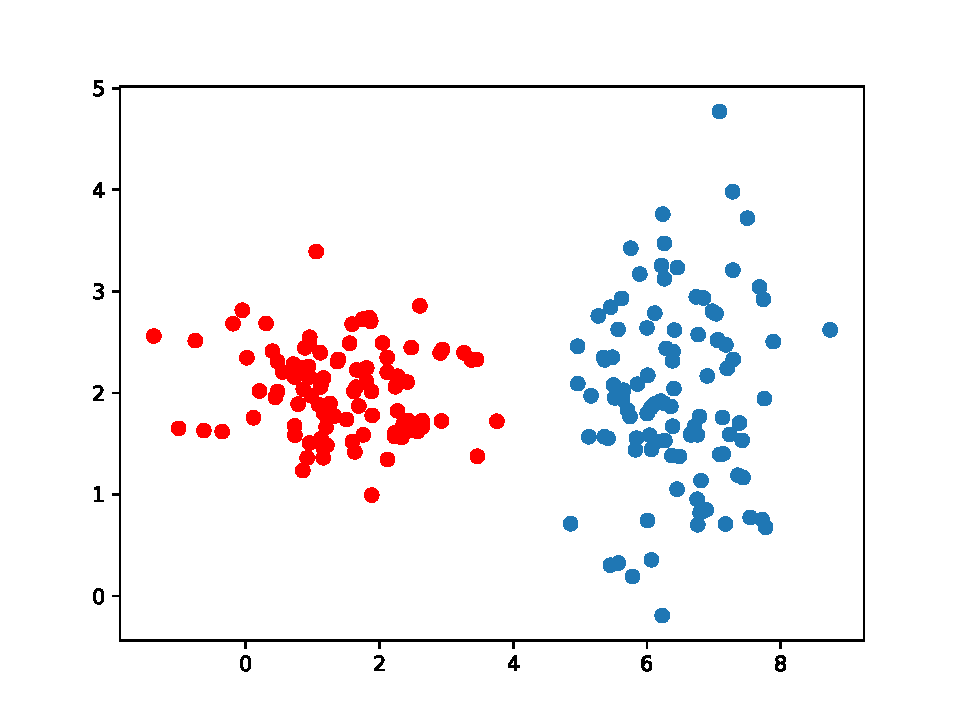
\includegraphics[width=8cm]{simple.pdf}
        \caption{Simple dataset}
        \end{figure}
        \begin{figure}[H]
        \centering
        \cleardoublepage
        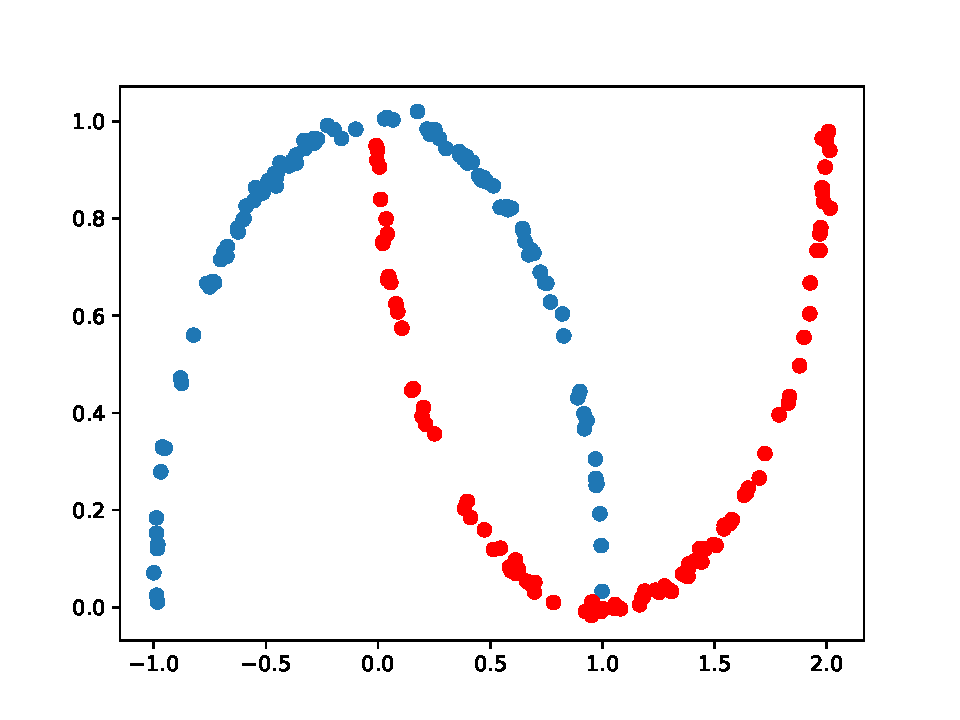
\includegraphics[width=8cm]{moon.pdf}
        \caption{Moon dataset}
        \end{figure}
    \end{solution}
  
 \end{nexercise}
 
 \cleardoublepage
 \begin{nexercise}{Support Vector Machine - Primal Problem}
 \par
 \begin{solution} 2.
        \begin{figure}[H]
        \centering
        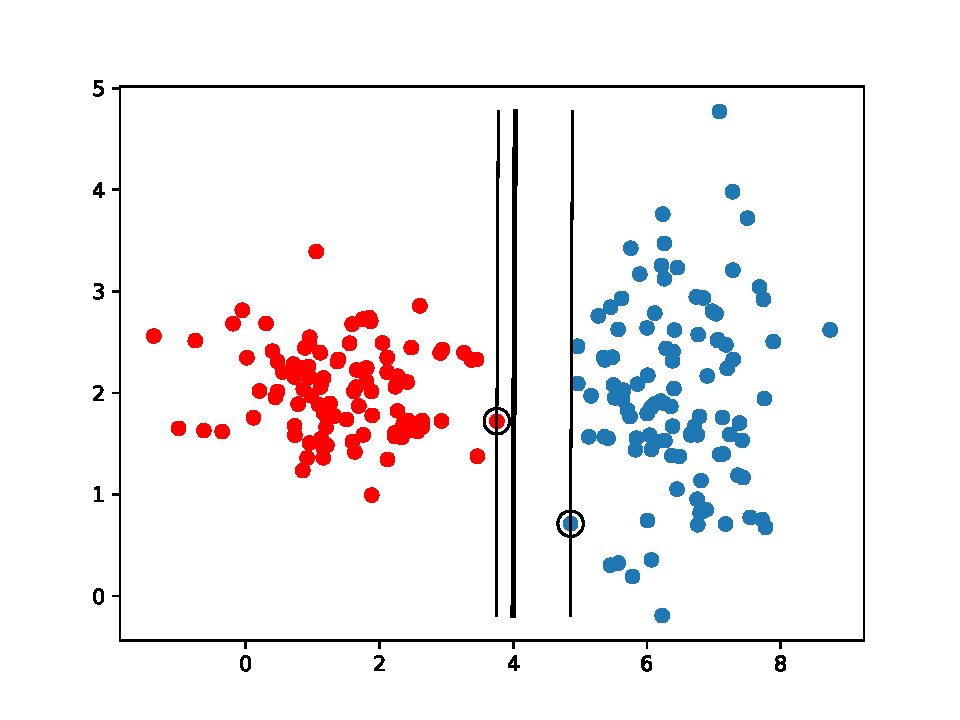
\includegraphics[width=13cm]{simple-line.pdf}
        \caption{First dataset, SVM}
        \centering
        \cleardoublepage
        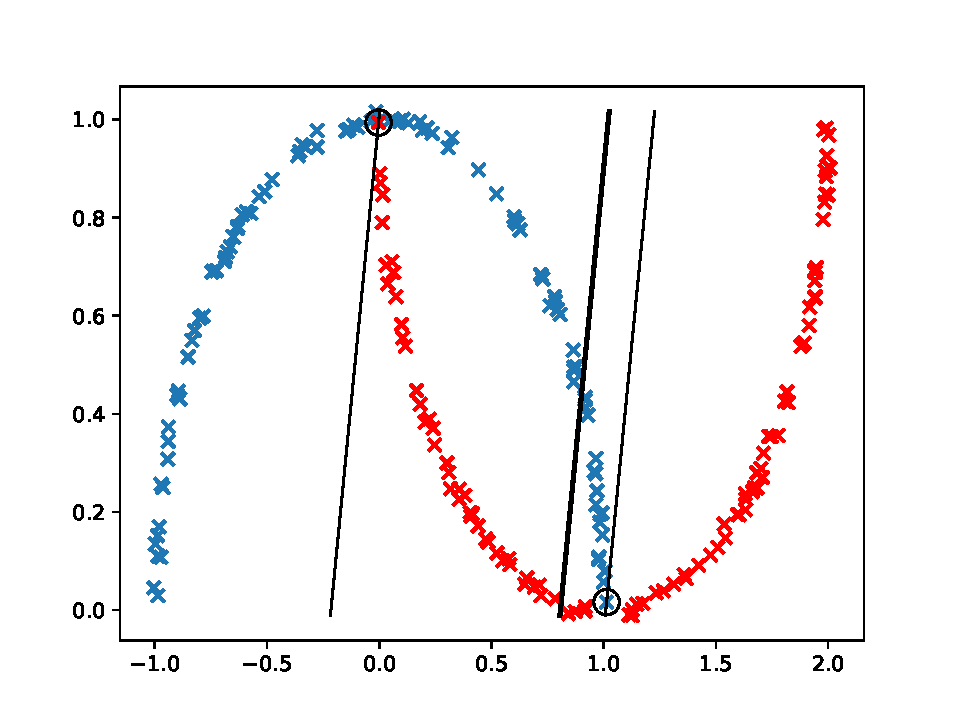
\includegraphics[width=10cm]{moon-line.pdf}
        \caption{Halfmoon dataset, SVM}
        \end{figure}
    
 
 We can notice that in the first example the SVM machine is clearly able to divide the two data sets. The space, in fact, is linearly separable.
 
 In the second example we notice that the SVM is not able to separate the two data sets. This space is in fact non-linearly separable so we need another, non-linear function in order to properly split the data.
 
  
 \end{solution}
 --------------------
 \end{nexercise}
 \begin{nexercise}{SVM - Dual Problem}
 \begin{solution}1.
 
 \begin{align*}
  ||\bm{\widetilde w}^{2}_{M}|| = \bm{\widetilde w}^{T}\bm{M}\bm{\widetilde w} = 10^{-6} w^{2}_{0}+\sum_{n=1}^{N}w_{m}^{2}
  \end{align*}
  \begin{align*}
      \frac{\partial }{\partial w_{0}} \frac{1}{2}||\bm{w}^{2}_{M}|| = 10^{-6}w_{0}
  \end{align*}
  \begin{align*}
      10^{-6}w_{0}-\sum_{n=1}^{N}t_{n}a_{n} \stackrel{!}{=} 0 
  \end{align*}
  \begin{align*}
      w_{0} = 10^{6}\sum_{n=1}^{N}t_{n}a_{n} = 10^{6}\sum_{n=1}^{N}t_{n}a_{n}\underbrace{\phi^{0}(x_{n})}_\text{=1}
  \end{align*}
  so we can rewrite the vector $\bm{\widetilde w}$ as
  \begin{align*}
      \bm{\widetilde w} = \sum_{n=1}^{N}t_{n}a_{n}\bm{M}^{-1}\bm{\phi}(x_{n})
  \end{align*}
  Considering $\bm{\widetilde w} = (b, \bm{w})$ and substituting we will end up with
  \begin{gather*}
       L(\bm{\widetilde w},a)=\frac{1}{2}\bm{\widetilde w}^{T}\bm{M}\bm{\widetilde w}+\sum_{n=1}^{N}a_{n}(1-t_{n}\bm{\widetilde w}^{T}\bm{\phi}(x_{n})) =  
       \\
       \frac{1}{2}(\bm{M}^{-1}\sum_{n=1}^{N}a_{n}t_{n}\bm{\phi}(x_{n}))^{T}\bm{M}(\bm{M}^{-1}\sum_{n=1}^{N}a_{n}t_{n}\bm{\phi}(x_{n})+  \sum_{n=1}^{N}a_{n}-\sum_{n=1}^{N}\sum_{m=1}^{N}a_{n}a_{m}t_{n}t_{m}(\bm{\phi}(x_{n}))^{T}\bm{M}\bm{\phi}(x_{m}) = \\
    \end{gather*}
        Finally we have
   \begin{align*}
        \sum_{n=1}^{N}a_{n}-\frac{1}{2}\sum_{n=1}^{N}\sum_{m=1}^{N}a_{n}a_{m}t_{n}t_{m}(\bm{\phi}(x_{n}))^{T}\bm{M}\bm{\phi}(\bm{x}_{n})
  \end{align*}
  \end{solution}
 
 \end{nexercise}
 
 \begin{solution}2.
 
 In order to compute the gradient, we split the sums in the following way:
 
 \begin{gather*}
     \nabla D(a) = \frac{\partial}{\partial a_{k}}( \sum_{n = 1, n \neq k}a_{n} + a_{k}-\frac{1}{2}\sum_{n=1, n\neq k}^{N}\sum_{m=1, m\neq k}^{N}a_{n}a_{m}t_{n}t_{m}k(\bm{x}_{n}, \bm{x}_{m})-\frac{1}{2}a_{k}t_{k}\sum_{n=1, n\neq k}^{N}a_{n}t_{n}k(\bm{x}_{n}, \bm{x}_{k}) + \\
     -\frac{1}{2}a_{k}t_{k}\sum_{m=1, n\neq k}^{N}a_{m}t_{m}k(\bm{x}_{k}, \bm{x}_{m})-\frac{1}{2}a_{k}^{2}t_{k}^{2}k(\bm{x}_{k}, \bm{x}_{k}))
 \end{gather*}
 So, computing the partial derivative we obtain:
 \begin{gather*}
     \nabla D(a) = 0+1-0-\frac{1}{2}t_{k}\sum_{n=1, n\neq k}^{N}a_{n}t_{n}k(\bm{x}_{n}, \bm{x}_{k})-\frac{1}{2}t_{k}\sum_{m=1, m \neq k}^{N}a_{m}t_{m}k(\bm{x}_{m}, \bm{x}_{k})-a_{k}t_{k}^{2}k(\bm{x}_{k}, \bm{x}_{k}) \\
     \nabla D(a) = 1-\frac{1}{2}t_{k}\sum_{n=1, n\neq k}^{N}a_{n}t_{n}k(\bm{x}_{n}, \bm{x}_{k})-\frac{1}{2}t_{k}\sum_{m=1, m \neq k}^{N}a_{m}t_{m}k(\bm{x}_{m}, \bm{x}_{k})-a_{k}t_{k}^{2}k(\bm{x}_{k}, \bm{x}_{k}) 
 \end{gather*}
 \end{solution}
 
 \begin{solution}3. 
 \begin{figure}[H]
        \centering
        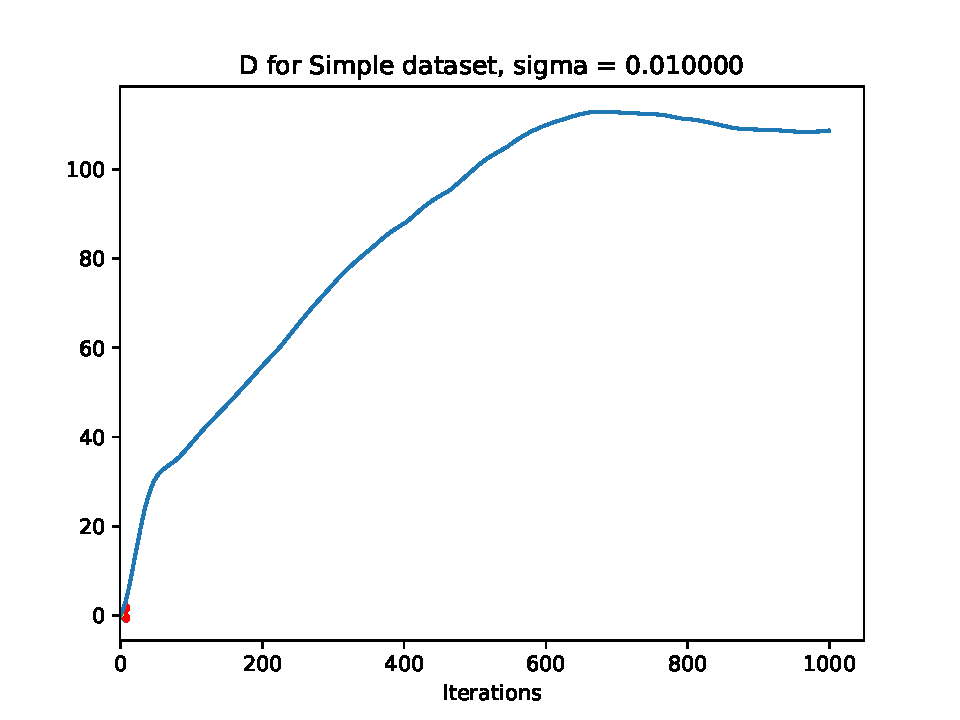
\includegraphics[width=10cm]{simple_D_iterations_s0.01.pdf}
        \end{figure}
 \begin{figure}[H]
        \centering
        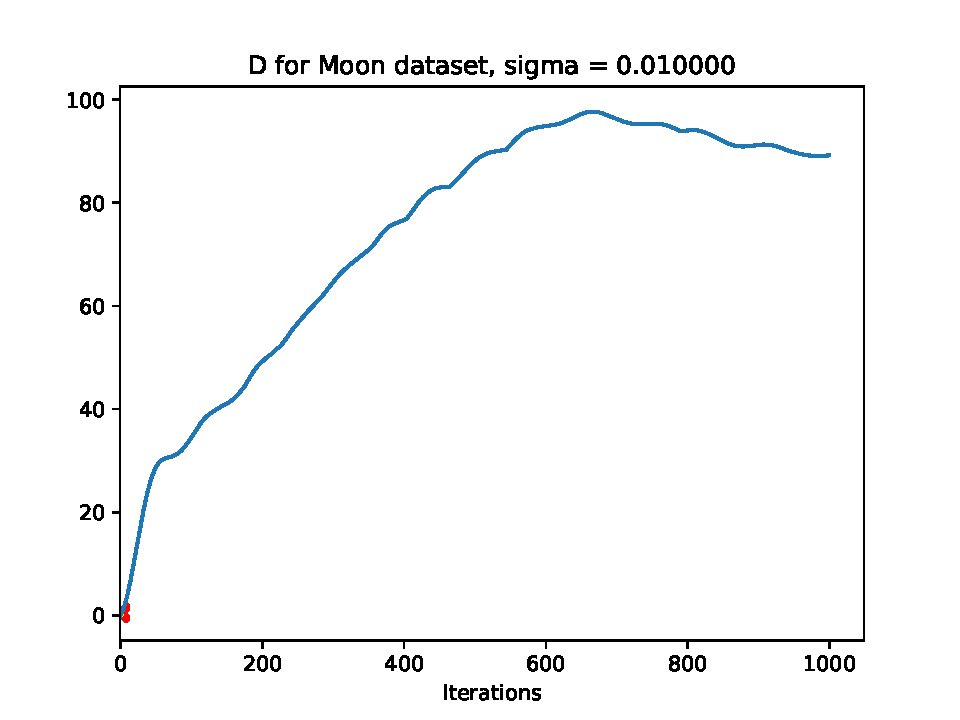
\includegraphics[width=10cm]{moon_D_iterations_s0.01.pdf}
        \end{figure}
 \begin{figure}[H]
        \centering
        \includegraphics[width=10cm]{simple_D_iterations.pdf}
        \end{figure}
 \begin{figure}[H]
        \centering
        \includegraphics[width=10cm]{moon_D_iterations.pdf}
        \end{figure}
        
        As we increase sigma, D converges faster. We also notice that for smaller $\sigma$ in the Moon Dataset the convergence is slightly slower, probably due to the higher complexity of the problem - non linearly separable vs a linearly separable one.
        \\*
        Here the plots for the decision boundaries: 
 \begin{figure}[H]
        \centering
        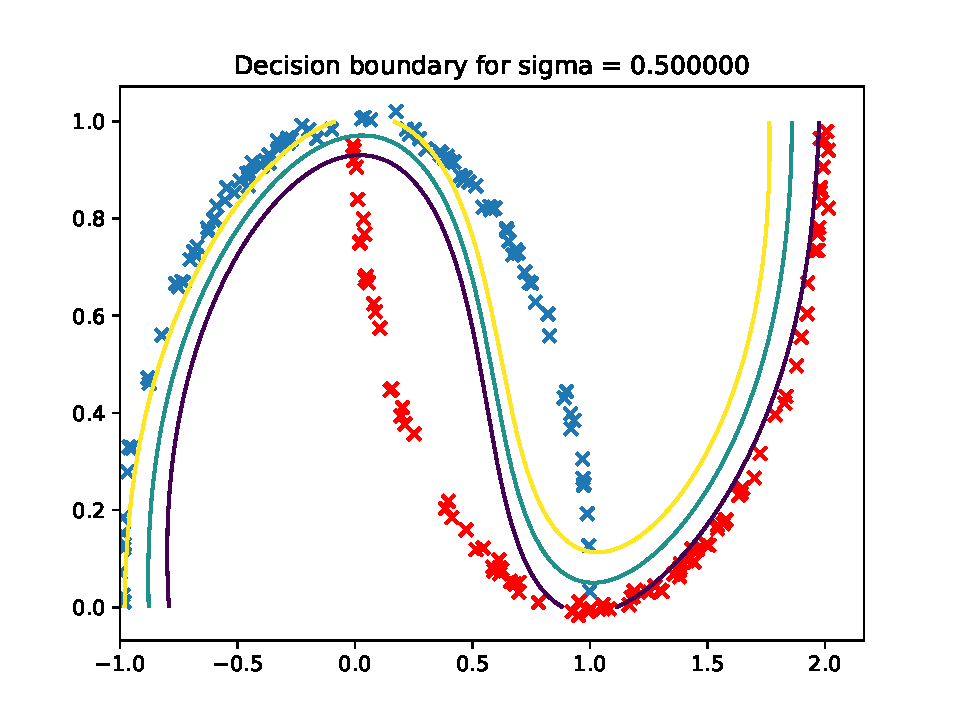
\includegraphics[width=10cm]{decision_boundary_2.pdf}
        \end{figure}
 \begin{figure}[H]
        \centering
        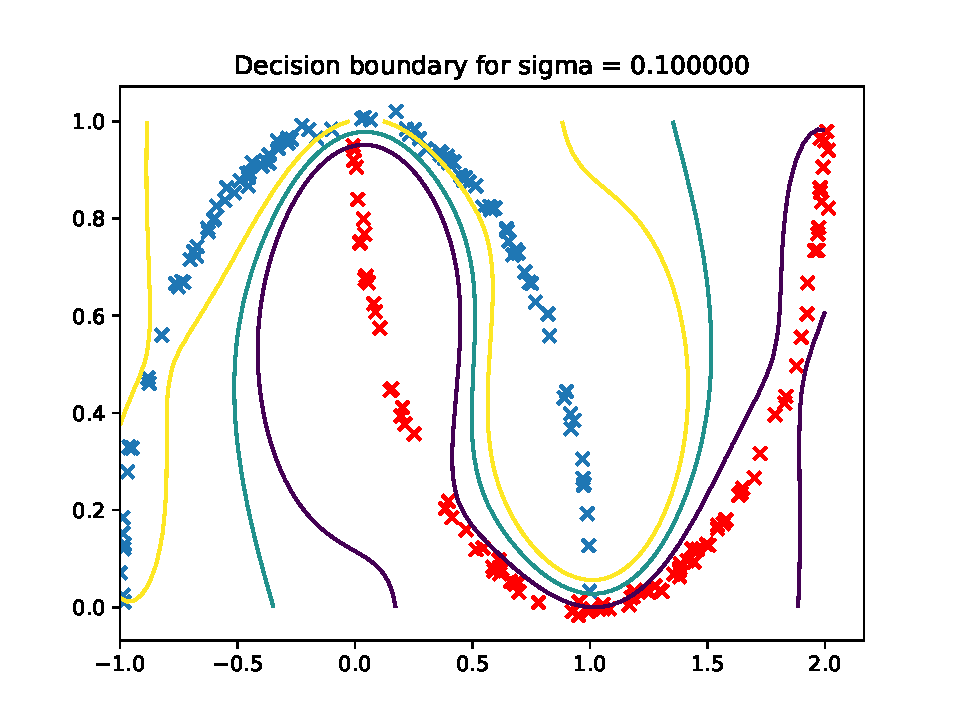
\includegraphics[width=10cm]{decision_boundary_0.pdf}
        \end{figure}
 \begin{figure}[H]
        \centering
        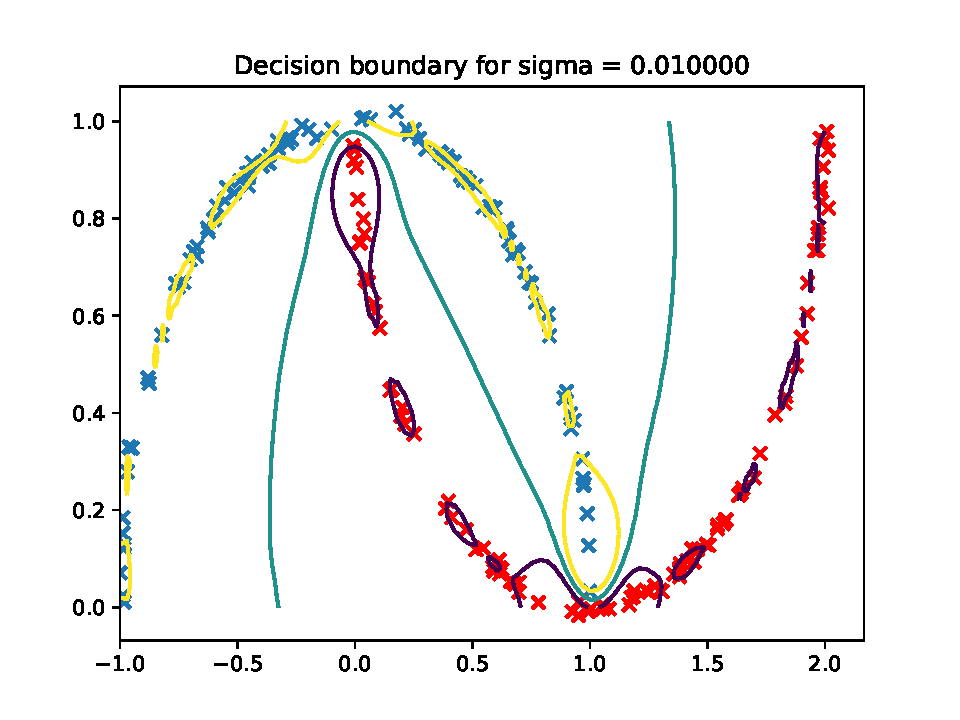
\includegraphics[width=10cm]{decision_boundary_1.pdf}
        \end{figure}
 \end{solution}
\end{document}
